Since the hounds will always win with optimal play from both sides, we can
use the percentage of wins from the hounds as a measure of performance. If
the hound win the majority of the games, then we can assume that the system is
fully trained. Therefore we decided to use this as a measure of performance. 

Graphs with the percentage of wins for the hounds for different
configurations can be found in \autoref{fig:dat}. Not all lines are visible
in \autoref{fig:r10000}, \autoref{fig:r100000}, and \autoref{fig:r5000000},
since the performance is so similar for different values of $\gamma$ that
they all lay on the same line and are therefore masked beneath eachother.

\begin{figure}[bt]
    \centering
    \begin{subfigure}{0.49\textwidth}
        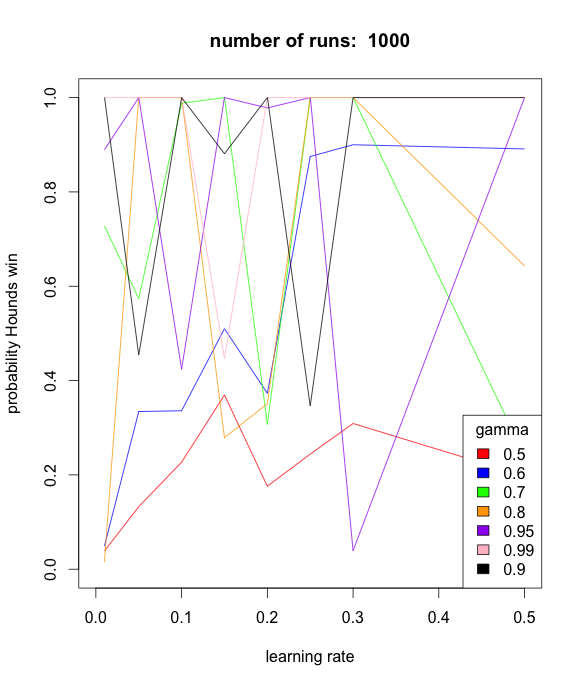
\includegraphics[width=\textwidth]{r1000}
        \caption{The percentage of wins for the hounds for different values
            of $\eta$ and $\gamma$ for 1000 runs}
        \label{fig:r1000}
    \end{subfigure}
    ~
    \begin{subfigure}{0.49\textwidth}
        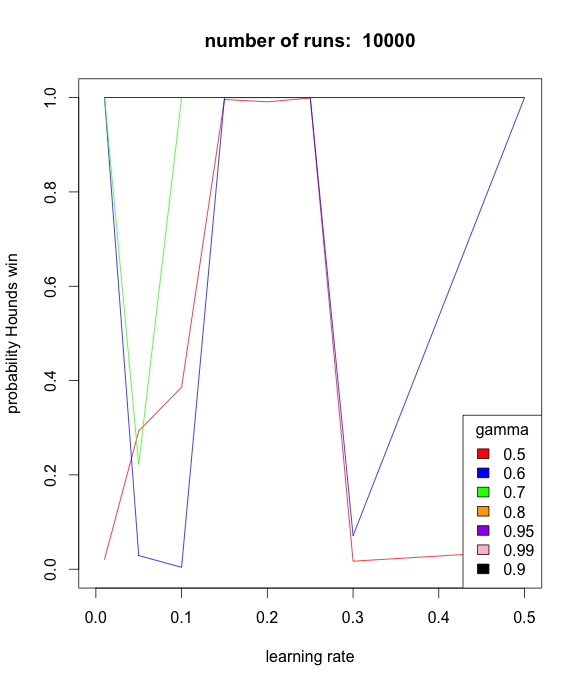
\includegraphics[width=\textwidth]{r10000}
        \caption{The percentage of wins for the hounds for different values
            of $\eta$ and $\gamma$ for 10000 runs}
        \label{fig:r10000}
    \end{subfigure}
    
    \begin{subfigure}{0.49\textwidth}
        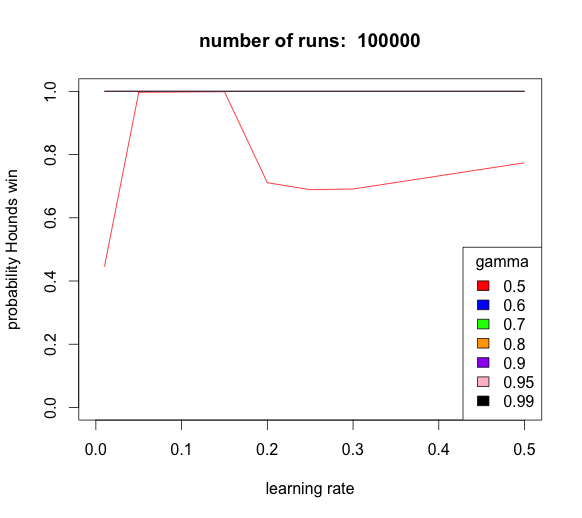
\includegraphics[width=\textwidth]{r100000}
        \caption{The percentage of wins for the hounds for different values
            of $\eta$ and $\gamma$ for 100000 runs}
        \label{fig:r100000}
    \end{subfigure}
    ~
    \begin{subfigure}{0.49\textwidth}
        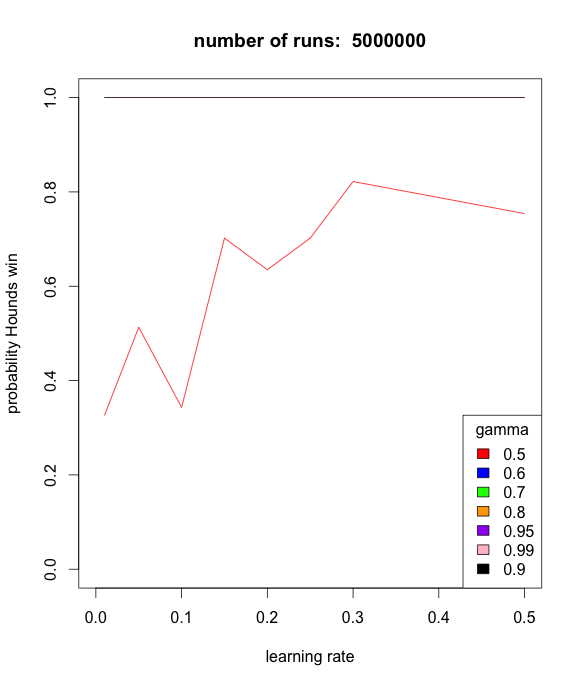
\includegraphics[width=\textwidth]{r5000000}
        \caption{The percentage of wins for the hounds for different values
            of $\eta$ and $\gamma$ for 5000000 runs}
        \label{fig:r5000000}
    \end{subfigure}
    \caption{The percentage of hounds wins for several configurations}
    \label{fig:dat}
\end{figure}

In the graphs we can see that after about 1000 training runs, for values of
$\gamma$ higher than $0.8$ and all values of $\eta$, the hounds always win.
From 10000 training runs and higher, this even goes for values of $\gamma$
of $0.6$ and higher. Here we can clearly see the effect of the discount
factor, if we have a lower discount factor, and therefore take a shorter
period of time into account, we have to train the system for longer than
when we focus more on the long run and therefore include more games.

What we can also see from \autoref{fig:r100000} and \autoref{fig:r5000000}
is that there is no difference in performance for all values of $\gamma$
higher than $0.6$ for this training time. That means that after 100000
training runs, one can stop training the system. For higher values of
$\gamma$, the system is already trained in 10000 training steps
(\autoref{fig:r10000})

We can also see that the value of $\eta$ does not have a large influence on
the eventual performance. This is not that unexpected, since the learning
rate is lowered over time, so for all values of $\eta$ it tends to 0 in
update proportional to the number of runs used for training and the
starting value of $\eta$. This means that after a few runs all values of
$\eta$ become similar.

To further see the influence of the paramters on the performance, we
constructed a linear model that can predict the performance based on the
parameters given. This model gives us similar results as we could see from
the graphs, with a high significance for the discount factor ($p < 1 \times
10 ^ {-11}$) and the number of runs ($p < 1 \times 10 ^ {-6}$), while the
value for the learning rate is not significant ($p = 0.281$). From this we
can confirm our suspicion that the value of the learning rate does not have a
great influence over the eventual performance.

